% Architecture diagrams of Meridian M0 and of the evaluation pipeline, drawn from the code:
% meridian/model.py (MeridianConfig, DiagonalSSM, Encoder, Meridian), scripts/benchmark_vol.py
% (variant_cfg "M0", train_meridian, run_meridian_fold), scripts/score_vol_benchmark.py,
% scripts/benchmark_tail.py, scripts/forward_test.py. Counts come from generated/numbers.tex.
\documentclass[10pt]{article}
\usepackage[T1]{fontenc}
\usepackage{libertinus}
\usepackage[scaled=0.9]{inconsolata}
\usepackage{amsmath,amssymb}
\usepackage[a4paper,landscape,margin=1.3cm]{geometry}
\usepackage{tikz}
\usetikzlibrary{positioning,arrows.meta,fit,backgrounds,calc}
\usepackage[hidelinks]{hyperref}
\pagestyle{empty}
% generated by scripts/build_report_tex.py -- do not edit
\newcommand{\AblMOne}{0.3432}
\newcommand{\AblMThree}{0.3477}
\newcommand{\AblMTwo}{0.3430}
\newcommand{\AblMZero}{0.3404}
\newcommand{\AblRuntimeMin}{41}
\newcommand{\AblSeeds}{3}
\newcommand{\AssetBest}{QQQ}
\newcommand{\AssetBestPct}{$-12.6\%$}
\newcommand{\AssetWorst}{USDJPY}
\newcommand{\AssetWorstPct}{$-1.1\%$}
\newcommand{\BreadthMCI}{[-12.4, -2.1]}
\newcommand{\BreadthMP}{0.002}
\newcommand{\BreadthMPct}{$-7.1\%$}
\newcommand{\DataEnd}{2026-07-31}
\newcommand{\DataStart}{2007-01-01}
\newcommand{\DevDates}{1,901}
\newcommand{\DevEnd}{2018-12-31}
\newcommand{\DevMPct}{$-8.8\%$}
\newcommand{\DevStart}{2012-06-14}
\newcommand{\EmbargoDays}{22}
\newcommand{\Epochs}{8}
\newcommand{\FirstYear}{2012}
\newcommand{\Folds}{12}
\newcommand{\FwdCommit}{108f349}
\newcommand{\FwdFirstOrigin}{2026-10-30}
\newcommand{\FwdFrozen}{2026-11-01 16:19:03 UTC}
\newcommand{\FwdLastOrigin}{2026-11-02}
\newcommand{\FwdLogged}{26}
\newcommand{\FwdOrigins}{2}
\newcommand{\FwdPct}{$+13.0\%$}
\newcommand{\FwdPre}{26}
\newcommand{\FwdQH}{0.3201}
\newcommand{\FwdQM}{0.3617}
\newcommand{\FwdScoredAt}{2026-11-03 08:44:08 UTC}
\newcommand{\FwdScoredDates}{1}
\newcommand{\FwdScoredN}{11}
\newcommand{\FwdScoredOrigin}{2026-10-30}
\newcommand{\FwdTrainRows}{54,481}
\newcommand{\FwdTrainThrough}{2026-10-29}
\newcommand{\GitAhead}{5}
\newcommand{\GitHead}{0a6cfcc}
\newcommand{\GitMain}{ab041b0}
\newcommand{\HFiveP}{$<$0.001}
\newcommand{\HFivePct}{$-9.6\%$}
\newcommand{\HHFiveP}{0.203}
\newcommand{\HHOne}{$-3.1\%$}
\newcommand{\HHOneP}{0.076}
\newcommand{\HHTwoP}{0.369}
\newcommand{\HTwentyTwoP}{0.356}
\newcommand{\HTwentyTwoPct}{$-0.9\%$}
\newcommand{\HitMax}{68.3\%}
\newcommand{\HitMin}{62.3\%}
\newcommand{\HoldAssets}{11}
\newcommand{\HoldDates}{2,168}
\newcommand{\HoldEnd}{2026-06-29}
\newcommand{\HoldRows}{20,906}
\newcommand{\HoldStart}{2019-01-01}
\newcommand{\LastYear}{2026}
\newcommand{\MacroEnd}{2026-07-28}
\newcommand{\MacroStart}{2007-01-02}
\newcommand{\MinTrainDays}{1260}
\newcommand{\NClipped}{469}
\newcommand{\NScripts}{68}
\newcommand{\NStale}{36}
\newcommand{\NTests}{11}
\newcommand{\NWLag}{7}
\newcommand{\PowerEighty}{451}
\newcommand{\PowerEightyYears}{1.8}
\newcommand{\PowerFifty}{197}
\newcommand{\PowerFiftyMonths}{9}
\newcommand{\RawComboCI}{[-9.5, -4.9]}
\newcommand{\RawComboPct}{$-7.0\%$}
\newcommand{\RawHARQ}{0.3249}
\newcommand{\RawHARcalPct}{$+1.3\%$}
\newcommand{\RawMCI}{[-9.7, -4.5]}
\newcommand{\RawMCIHi}{$-4.5\%$}
\newcommand{\RawMP}{$<$0.001}
\newcommand{\RawMPct}{$-6.8\%$}
\newcommand{\RegCalmPct}{$-4.1\%$}
\newcommand{\RegNormalPct}{$-5.2\%$}
\newcommand{\RegStressPct}{$-14.1\%$}
\newcommand{\Seeds}{5}
\newcommand{\ShareDay}{61.2\%}
\newcommand{\ShareSixtyThree}{96.5\%}
\newcommand{\ShareTwenty}{86.6\%}
\newcommand{\ShareTwoFiftyTwo}{100.0\%}
\newcommand{\TCC}{11}
\newcommand{\TCCFive}{11}
\newcommand{\TCCOne}{11}
\newcommand{\TCCTwo}{11}
\newcommand{\TDQ}{10}
\newcommand{\TDQFive}{9}
\newcommand{\TDQOne}{10}
\newcommand{\TDQTwo}{10}
\newcommand{\TDevHAR}{-3.7832}
\newcommand{\TDevSel}{-3.7753}
\newcommand{\TESR}{0.98}
\newcommand{\TFZ}{-0.1218}
\newcommand{\TFZCI}{[-0.1533, -0.0949]}
\newcommand{\TFZP}{$<$0.001}
\newcommand{\TGNOneViol}{1.80\%}
\newcommand{\THSOne}{$+26.3\%$}
\newcommand{\THarDQ}{8}
\newcommand{\THarEVTDQ}{7}
\newcommand{\TKupFive}{11}
\newcommand{\TKupOne}{11}
\newcommand{\TKupTwo}{11}
\newcommand{\TRMOneViol}{2.10\%}
\newcommand{\TVFive}{$-5.1\%$}
\newcommand{\TVOne}{$-9.2\%$}
\newcommand{\TVOneCI}{[-12.7, -5.9]}
\newcommand{\TVOneP}{$<$0.001}
\newcommand{\TVTwo}{$-7.4\%$}
\newcommand{\TViolFive}{4.95\%}
\newcommand{\TViolOne}{0.96\%}
\newcommand{\TViolTwo}{2.49\%}
\newcommand{\TailDates}{2,168}
\newcommand{\TailEVTu}{0.90}
\newcommand{\TailGamma}{0.005}
\newcommand{\TailHS}{500}
\newcommand{\TailRef}{GJR-GARCH + FHS}
\newcommand{\TailRefit}{21}
\newcommand{\TailRows}{20,906}
\newcommand{\TailRuntime}{99}
\newcommand{\TailSel}{Meridian + EVT}
\newcommand{\TailZMin}{250}
\newcommand{\TailZWin}{1000}
\newcommand{\TestDays}{378}
\newcommand{\VComboCI}{[-12.4, -5.2]}
\newcommand{\VComboP}{$<$0.001}
\newcommand{\VComboPct}{$-8.2\%$}
\newcommand{\VComboQ}{0.3022}
\newcommand{\VComboWon}{11}
\newcommand{\VEGARCHCI}{[+8.1, +16.8]}
\newcommand{\VEGARCHP}{1.000}
\newcommand{\VEGARCHPct}{$+12.2\%$}
\newcommand{\VEGARCHQ}{0.3695}
\newcommand{\VEGARCHWon}{0}
\newcommand{\VEWMACI}{[+7.9, +21.8]}
\newcommand{\VEWMAP}{1.000}
\newcommand{\VEWMAPct}{$+14.1\%$}
\newcommand{\VEWMAQ}{0.3758}
\newcommand{\VEWMAWon}{0}
\newcommand{\VGARCHCI}{[+11.0, +18.6]}
\newcommand{\VGARCHP}{1.000}
\newcommand{\VGARCHPct}{$+14.9\%$}
\newcommand{\VGARCHQ}{0.3782}
\newcommand{\VGARCHWon}{0}
\newcommand{\VGJRCI}{[+9.9, +18.9]}
\newcommand{\VGJRP}{1.000}
\newcommand{\VGJRPct}{$+14.1\%$}
\newcommand{\VGJRQ}{0.3758}
\newcommand{\VGJRWon}{0}
\newcommand{\VHARLGBMCI}{[-9.3, -3.1]}
\newcommand{\VHARLGBMP}{$<$0.001}
\newcommand{\VHARLGBMPct}{$-5.7\%$}
\newcommand{\VHARLGBMQ}{0.3105}
\newcommand{\VHARLGBMWon}{10}
\newcommand{\VHARQ}{0.3292}
\newcommand{\VHARXCI}{[-7.7, -2.9]}
\newcommand{\VHARXP}{$<$0.001}
\newcommand{\VHARXPct}{$-5.0\%$}
\newcommand{\VHARXQ}{0.3126}
\newcommand{\VHARXWon}{10}
\newcommand{\VLGBMCI}{[-9.3, -2.5]}
\newcommand{\VLGBMP}{$<$0.001}
\newcommand{\VLGBMPct}{$-5.3\%$}
\newcommand{\VLGBMQ}{0.3118}
\newcommand{\VLGBMWon}{10}
\newcommand{\VLHARCI}{[-5.4, -0.5]}
\newcommand{\VLHARP}{0.011}
\newcommand{\VLHARPct}{$-2.7\%$}
\newcommand{\VLHARQ}{0.3204}
\newcommand{\VLHARWon}{10}
\newcommand{\VMCI}{[-11.3, -4.7]}
\newcommand{\VMP}{$<$0.001}
\newcommand{\VMPct}{$-7.5\%$}
\newcommand{\VMQ}{0.3045}
\newcommand{\VMWon}{11}
\newcommand{\VRFCI}{[-6.8, -1.4]}
\newcommand{\VRFP}{$<$0.001}
\newcommand{\VRFPct}{$-3.7\%$}
\newcommand{\VRFQ}{0.3171}
\newcommand{\VRFWon}{11}
\newcommand{\VRWCI}{[+12.9, +24.7]}
\newcommand{\VRWP}{1.000}
\newcommand{\VRWPct}{$+18.0\%$}
\newcommand{\VRWQ}{0.3884}
\newcommand{\VRWWon}{0}
\newcommand{\VRidgeCI}{[-8.7, -2.1]}
\newcommand{\VRidgeP}{$<$0.001}
\newcommand{\VRidgePct}{$-4.9\%$}
\newcommand{\VRidgeQ}{0.3132}
\newcommand{\VRidgeWon}{9}
\newcommand{\VTMCI}{[+0.3, +6.1]}
\newcommand{\VTMP}{0.957}
\newcommand{\VTMPct}{$+3.0\%$}
\newcommand{\VTMQ}{0.3392}
\newcommand{\VTMWon}{3}
\newcommand{\VolRunCommit}{ab041b0}
\newcommand{\VolRuntimeMin}{18}
\newcommand{\WorstYear}{2026}
\newcommand{\WorstYearPct}{$+0.04\%$}
\newcommand{\YearsTotal}{15}
\newcommand{\YearsWon}{14}


\definecolor{accent}{HTML}{1D4E89}
\definecolor{inp}{HTML}{E8EEF6}
\definecolor{enc}{HTML}{DCE8F5}
\definecolor{head}{HTML}{E3F2E8}
\definecolor{aux}{HTML}{FFF4E0}
\definecolor{jepa}{HTML}{F1E8F7}
\definecolor{loss}{HTML}{FBEAEA}
\definecolor{grey}{HTML}{F2F2F2}
\definecolor{ink}{HTML}{1F2933}
\definecolor{muted}{HTML}{52606D}

\tikzset{
  box/.style={draw=ink!70, rounded corners=2pt, align=center, font=\small, inner sep=3pt,
              minimum height=9mm, line width=0.5pt},
  op/.style={draw=ink!70, circle, inner sep=0.8pt, font=\small, line width=0.5pt, fill=white},
  arr/.style={-{Stealth[length=2.2mm]}, line width=0.6pt, draw=ink!80},
  darr/.style={arr, dashed, draw=ink!40},
  dim/.style={font=\scriptsize\itshape, text=muted},
  group/.style={draw=accent!60, dashed, rounded corners=4pt, line width=0.6pt},
  ttl/.style={font=\scriptsize\bfseries, text=accent},
}
\newcommand{\sub}[1]{\\[-1pt]{\scriptsize #1}}

\begin{document}

% =====================================================================================
% PAGE 1 -- the network
% =====================================================================================
\noindent{\Large\bfseries\color{accent} Meridian M0 --- network architecture as used in the audited benchmark}\\[1pt]
{\small\color{muted} Source: \texttt{meridian/model.py} with configuration \texttt{variant\_cfg("M0")} in
\texttt{scripts/benchmark\_vol.py}. Shapes: $B$ = batch, 32 days, 15 features, width 64, SSM state 64.}

\vspace{2mm}
\begin{center}
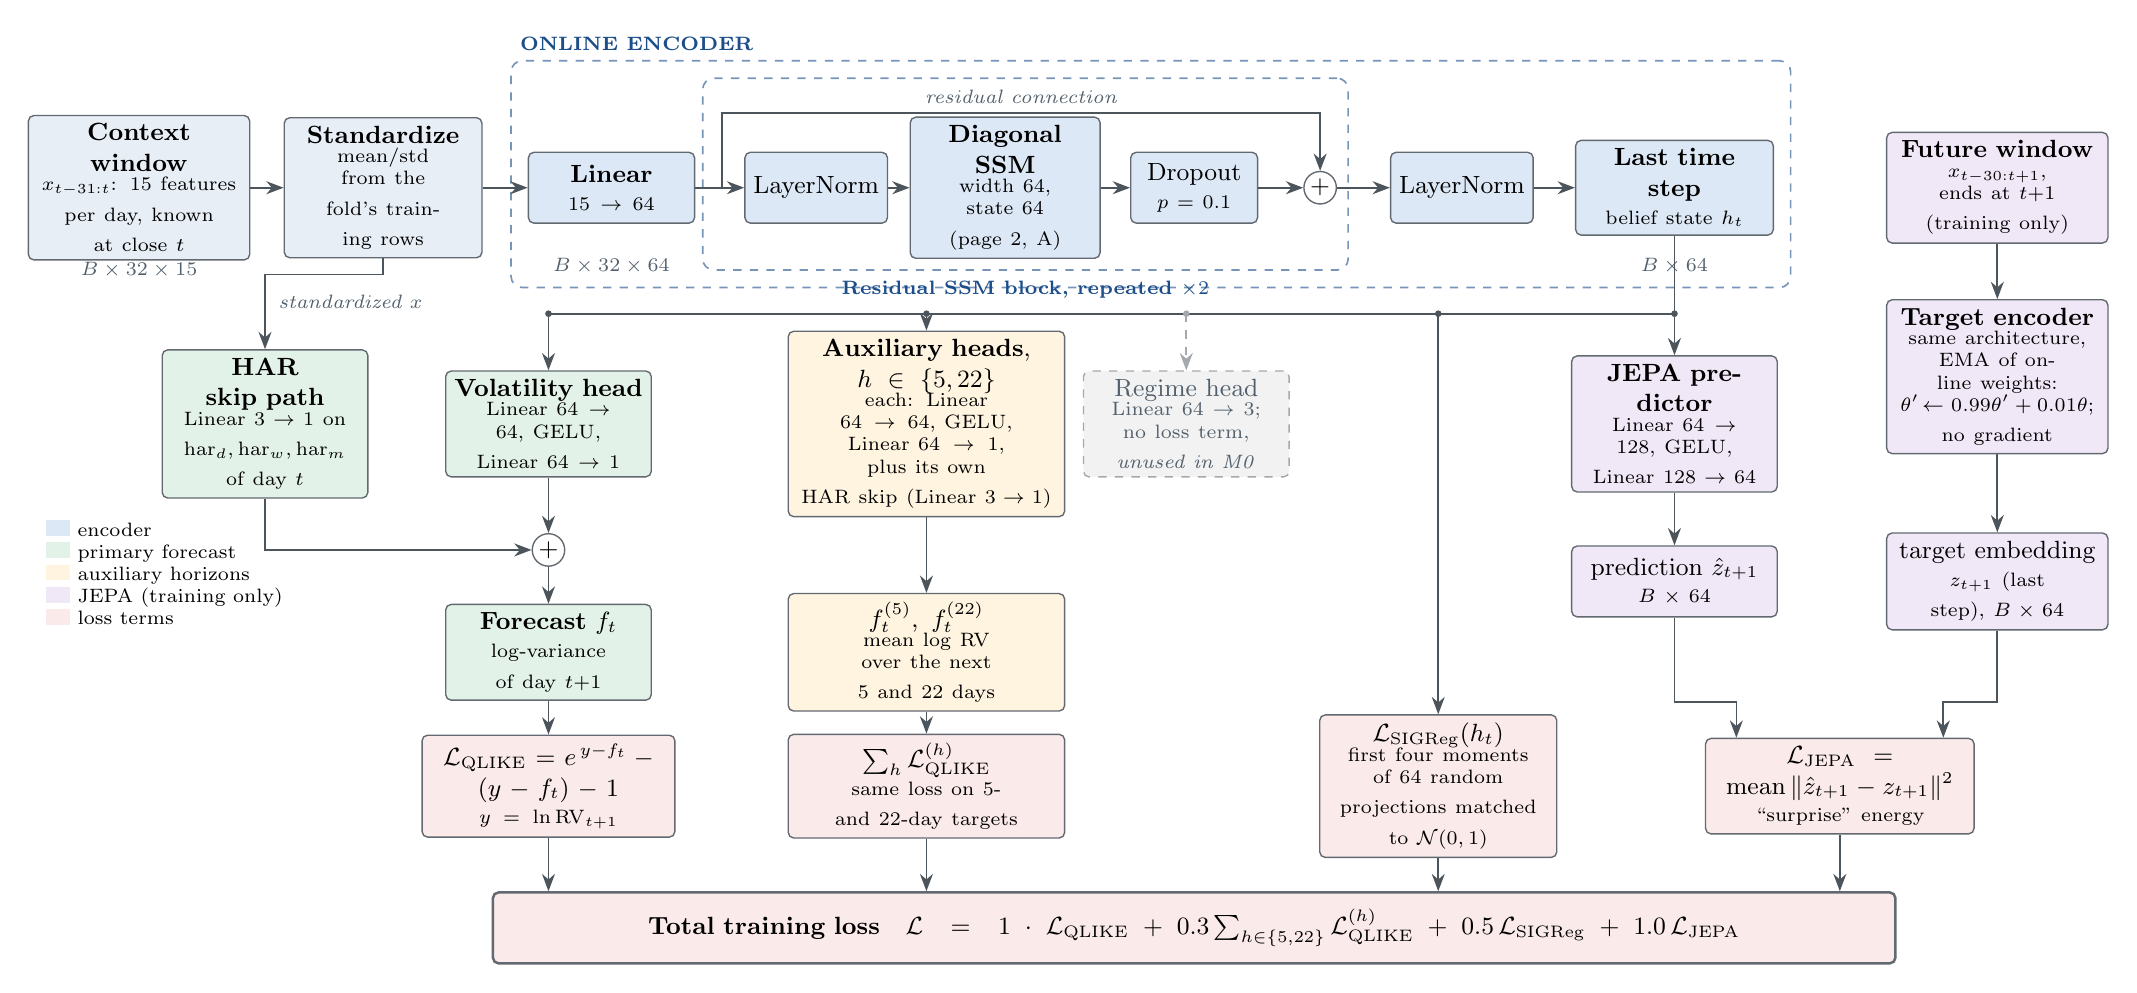
\begin{tikzpicture}[x=1cm,y=1cm]
% ---------------- row A: input and encoder
\node[box, fill=inp, text width=2.6cm] (x) at (0,0) {\textbf{Context window}\sub{$x_{t-31:t}$: 15 features\\per day, known at close $t$}};
\node[dim] at (0,-1.05) {$B\times32\times15$};
\node[box, fill=inp, text width=2.3cm] (sc) at (3.1,0) {\textbf{Standardize}\sub{mean/std from the\\fold's training rows}};
\node[box, fill=enc, text width=1.9cm] (lin) at (6.0,0) {\textbf{Linear}\sub{$15\to64$}};
\node[dim] at (6.0,-1.0) {$B\times32\times64$};
\node[box, fill=enc, text width=1.6cm] (ln1) at (8.6,0) {LayerNorm};
\node[box, fill=enc, text width=2.2cm] (ssm) at (11.0,0) {\textbf{Diagonal SSM}\sub{width 64, state 64\\(page 2, A)}};
\node[box, fill=enc, text width=1.4cm] (do) at (13.4,0) {Dropout\sub{$p=0.1$}};
\node[op] (plus) at (15.0,0) {$+$};
\node[box, fill=enc, text width=1.6cm] (lnf) at (16.8,0) {LayerNorm};
\node[box, fill=enc, text width=2.3cm] (last) at (19.5,0) {\textbf{Last time step}\sub{belief state $h_t$}};
\node[dim] at (19.5,-1.0) {$B\times64$};

\draw[arr] (x)--(sc); \draw[arr] (sc)--(lin); \draw[arr] (lin)--(ln1); \draw[arr] (ln1)--(ssm);
\draw[arr] (ssm)--(do); \draw[arr] (do)--(plus); \draw[arr] (plus)--(lnf); \draw[arr] (lnf)--(last);
\draw[arr] (7.4,0) -- (7.4,0.95) -| (plus.north);
\node[dim, anchor=south] at (11.2,0.95) {residual connection};
\begin{scope}[on background layer]
\node[group, fit={(ln1)(ssm)(do)(plus)(7.3,1.25)}, inner sep=4pt] (blk) {};
\node[group, fit={(lin)(blk)(last)(6.0,-1.05)}, inner sep=6pt] (encg) {};
\end{scope}
\node[ttl, anchor=north] at (blk.south) {Residual SSM block, repeated $\times2$};
\node[ttl, anchor=south west] at (encg.north west) {ONLINE ENCODER};

% ---------------- JEPA target branch (right)
\node[box, fill=jepa, text width=2.6cm] (xf) at (23.6,0) {\textbf{Future window}\sub{$x_{t-30:t+1}$, ends at $t{+}1$\\(training only)}};
\node[box, fill=jepa, text width=2.6cm] (te) at (23.6,-2.4) {\textbf{Target encoder}\sub{same architecture,\\EMA of online weights:\\$\theta'\!\leftarrow 0.99\theta'+0.01\theta$;\\no gradient}};
\node[box, fill=jepa, text width=2.6cm] (z) at (23.6,-5.0) {target embedding\sub{$z_{t+1}$ (last step), $B\times64$}};
\draw[arr] (xf)--(te); \draw[arr] (te)--(z);

% ---------------- bus from h_t
\draw[line width=0.6pt, draw=ink!80] (last.south) -- (19.5,-1.6) -- (5.2,-1.6);
\foreach \xx in {5.2, 10.0, 16.5, 19.5} \fill[ink!80] (\xx,-1.6) circle (1.2pt);

% ---------------- heads
\node[box, fill=head, text width=2.4cm] (skip) at (1.6,-3.0) {\textbf{HAR skip path}\sub{Linear $3\to1$ on\\$\mathrm{har}_d,\mathrm{har}_w,\mathrm{har}_m$ of day $t$}};
\node[box, fill=head, text width=2.4cm] (vh) at (5.2,-3.0) {\textbf{Volatility head}\sub{Linear $64\to64$, GELU,\\Linear $64\to1$}};
\node[op] (vplus) at (5.2,-4.6) {$+$};
\node[box, fill=head, text width=2.4cm] (f) at (5.2,-5.9) {\textbf{Forecast $f_t$}\sub{log-variance of day $t{+}1$}};
\draw[arr] (5.2,-1.6)--(vh.north); \draw[arr] (vh)--(vplus); \draw[arr] (skip.south) |- (vplus.west);
\draw[arr] (vplus)--(f);
\draw[arr] (sc.south) -- (3.1,-1.1) -| (skip.north);
\node[dim, anchor=west] at (1.65,-1.45) {standardized $x$};

\node[box, fill=aux, text width=3.3cm] (ah) at (10.0,-3.0) {\textbf{Auxiliary heads}, $h\in\{5,22\}$\sub{each: Linear $64\to64$, GELU,\\Linear $64\to1$, plus its own\\HAR skip (Linear $3\to1$)}};
\node[box, fill=aux, text width=3.3cm] (af) at (10.0,-5.9) {$f^{(5)}_t,\ f^{(22)}_t$\sub{mean log RV over the next\\5 and 22 days}};
\draw[arr] (10.0,-1.6)--(ah.north); \draw[arr] (ah)--(af);

\node[box, fill=grey, draw=ink!40, dashed, text=muted, text width=2.4cm] (rh) at (13.3,-3.0) {Regime head\sub{Linear $64\to3$;\\no loss term,\\\emph{unused in M0}}};
\draw[darr] (13.3,-1.6)--(rh.north);
\fill[ink!40] (13.3,-1.6) circle (1.2pt);

\node[box, fill=jepa, text width=2.4cm] (pred) at (19.5,-3.0) {\textbf{JEPA predictor}\sub{Linear $64\to128$, GELU,\\Linear $128\to64$}};
\node[box, fill=jepa, text width=2.4cm] (zh) at (19.5,-5.0) {prediction $\hat z_{t+1}$\sub{$B\times64$}};
\draw[arr] (19.5,-1.6)--(pred.north); \draw[arr] (pred)--(zh);

% ---------------- losses
\node[box, fill=loss, text width=3.0cm] (lq) at (5.2,-7.6) {$\mathcal{L}_{\mathrm{QLIKE}}=e^{\,y-f_t}-(y-f_t)-1$\sub{$y=\ln\mathrm{RV}_{t+1}$}};
\node[box, fill=loss, text width=3.3cm] (la) at (10.0,-7.6) {$\sum_{h}\mathcal{L}^{(h)}_{\mathrm{QLIKE}}$\sub{same loss on 5- and 22-day targets}};
\node[box, fill=loss, text width=2.8cm] (ls) at (16.5,-7.6) {$\mathcal{L}_{\mathrm{SIGReg}}(h_t)$\sub{first four moments of 64 random\\projections matched to $\mathcal{N}(0,1)$}};
\node[box, fill=loss, text width=3.2cm] (lj) at (21.6,-7.6) {$\mathcal{L}_{\mathrm{JEPA}}=\mathrm{mean}\,\lVert\hat z_{t+1}-z_{t+1}\rVert^2$\sub{``surprise'' energy}};
\draw[arr] (f)--(lq); \draw[arr] (af)--(la);
\draw[arr] (16.5,-1.6)--(ls.north);
\draw[arr] (zh.south) |- ($(lj.north west)+(0.4,0.45)$) -- ($(lj.north west)+(0.4,0)$);
\draw[arr] (z.south) |- ($(lj.north east)+(-0.4,0.45)$) -- ($(lj.north east)+(-0.4,0)$);

\node[box, fill=loss, line width=0.9pt, text width=17.6cm] (tot) at (13.4,-9.4)
 {\textbf{Total training loss}\quad
 $\mathcal{L}=1\cdot\mathcal{L}_{\mathrm{QLIKE}}+0.3\sum_{h\in\{5,22\}}\mathcal{L}^{(h)}_{\mathrm{QLIKE}}+0.5\,\mathcal{L}_{\mathrm{SIGReg}}+1.0\,\mathcal{L}_{\mathrm{JEPA}}$};
\foreach \n in {lq,la,ls,lj} \draw[arr] (\n.south) -- (\n.south |- tot.north);

% legend
\node[anchor=north west, font=\scriptsize, align=left] at (-1.3,-4.1) {
\tikz\fill[enc] (0,0) rectangle (3mm,2mm); encoder\\
\tikz\fill[head] (0,0) rectangle (3mm,2mm); primary forecast\\
\tikz\fill[aux] (0,0) rectangle (3mm,2mm); auxiliary horizons\\
\tikz\fill[jepa] (0,0) rectangle (3mm,2mm); JEPA (training only)\\
\tikz\fill[loss] (0,0) rectangle (3mm,2mm); loss terms};
\end{tikzpicture}
\end{center}

\vspace{-2mm}
{\small\noindent\textbf{What leaves the network.} Only $f_t$ is used as the volatility forecast ($f^{(5)}_t,f^{(22)}_t$ only for
the horizon tables). The JEPA branch, the target encoder and SIGReg act only during training.
\textbf{Ensemble.} \Seeds\ independently seeded copies are trained in every walk-forward fold, and the reported forecast is
the mean of their $f_t$. \textbf{Initialization.} The HAR skip paths start at the fold's HAR regression and the last layers of
the heads start at zero, so $f_t$ equals the HAR-RV forecast before training (page 2, B).}

\newpage
% =====================================================================================
% PAGE 2 -- SSM layer, HAR anchor, training loop
% =====================================================================================
\noindent{\Large\bfseries\color{accent} Inside the network: the SSM layer, the HAR-anchored start, the training loop}\\[1pt]
{\small\color{muted} Source: \texttt{DiagonalSSM}, \texttt{Encoder}, \texttt{Meridian.init\_har\_anchor} in
\texttt{meridian/model.py}; \texttt{train\_meridian}, \texttt{run\_meridian\_fold} in \texttt{scripts/benchmark\_vol.py}.}

\vspace{4mm}
\noindent
\begin{minipage}[t]{0.53\linewidth}
{\bfseries\color{accent} A. Diagonal linear state-space layer (one per residual block)}\\[3mm]
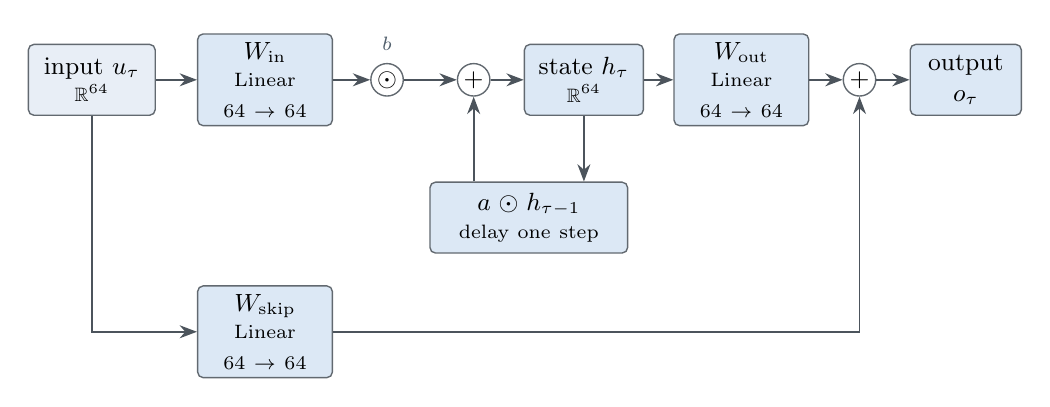
\begin{tikzpicture}[x=1cm,y=1cm]
\node[box, fill=inp, text width=1.4cm] (u) at (0,0) {input $u_\tau$\sub{$\mathbb{R}^{64}$}};
\node[box, fill=enc, text width=1.5cm] (win) at (2.2,0) {$W_{\mathrm{in}}$\sub{Linear $64\to64$}};
\node[op] (mb) at (3.75,0) {$\odot$};
\node[dim, anchor=south] at (3.75,0.25) {$b$};
\node[op] (sum) at (4.85,0) {$+$};
\node[box, fill=enc, text width=1.3cm] (h) at (6.25,0) {state $h_\tau$\sub{$\mathbb{R}^{64}$}};
\node[box, fill=enc, text width=1.5cm] (wout) at (8.25,0) {$W_{\mathrm{out}}$\sub{Linear $64\to64$}};
\node[op] (osum) at (9.75,0) {$+$};
\node[box, fill=enc, text width=1.2cm] (o) at (11.1,0) {output $o_\tau$};
\node[box, fill=enc, text width=2.3cm] (dec) at (5.55,-1.75) {$a\odot h_{\tau-1}$\sub{delay one step}};
\node[box, fill=enc, text width=1.5cm] (wsk) at (2.2,-3.2) {$W_{\mathrm{skip}}$\sub{Linear $64\to64$}};
\draw[arr] (u)--(win); \draw[arr] (win)--(mb); \draw[arr] (mb)--(sum); \draw[arr] (sum)--(h);
\draw[arr] (h)--(wout); \draw[arr] (wout)--(osum); \draw[arr] (osum)--(o);
\draw[arr] (h.south) -- (h.south |- dec.north);
\draw[arr] (dec.north -| sum) -- (sum.south);
\draw[arr] (u.south) |- (wsk.west);
\draw[arr] (wsk.east) -| (osum.south);
\end{tikzpicture}

\vspace{3mm}
{\small
\[
h_\tau = a\odot h_{\tau-1} + b\odot W_{\mathrm{in}}u_\tau,\qquad
o_\tau = W_{\mathrm{out}}h_\tau + W_{\mathrm{skip}}u_\tau,\qquad h_0=0,\quad \tau=1,\dots,32 .
\]
$a=\mathrm{sigmoid}(\alpha)$ is a learned decay per state channel, initialized with
$\alpha=\mathrm{linspace}(1,4)$, i.e.\ $a\in(0.73,\,0.98)$: each channel is a stable exponential memory with its own time
scale. $b$ is a learned input gain, initialized to 0.5. The recurrence is scanned sequentially over the 32 days. In the
encoder each layer is wrapped as $x\leftarrow x+\mathrm{Dropout}(\mathrm{SSM}(\mathrm{LayerNorm}(x)))$; two blocks are stacked
and followed by a final LayerNorm.}

\vspace{5mm}
{\bfseries\color{accent} B. HAR-anchored initialization (HARNet-style), every fold, every seed}\\[1mm]
{\small
\begin{enumerate}\itemsep1pt
\item Fit pooled HAR by OLS on the fold's core-asset training rows:
$\ln\mathrm{RV}_{t+1}=\beta_0+\beta_d\,\mathrm{har}_d+\beta_w\,\mathrm{har}_w+\beta_m\,\mathrm{har}_m$
(and the same regression for the 5- and 22-day targets).
\item Set the HAR skip path to weights $w=\beta_{1:3}\odot\sigma_{\mathrm{har}}$ and bias
$\beta_0+\beta_{1:3}^{\top}\mu_{\mathrm{har}}$, where $\mu_{\mathrm{har}},\sigma_{\mathrm{har}}$ are the scaler's statistics, so the
skip path reproduces HAR on standardized inputs.
\item Set the final linear layer of the volatility head and of both auxiliary heads to zero.
\end{enumerate}
Consequence: before the first gradient step, $f_t$ is exactly the HAR-RV forecast. Training only learns corrections to HAR.}
\end{minipage}\hfill
\begin{minipage}[t]{0.43\linewidth}
{\bfseries\color{accent} C. Training and forecasting in one walk-forward fold}\\[3mm]
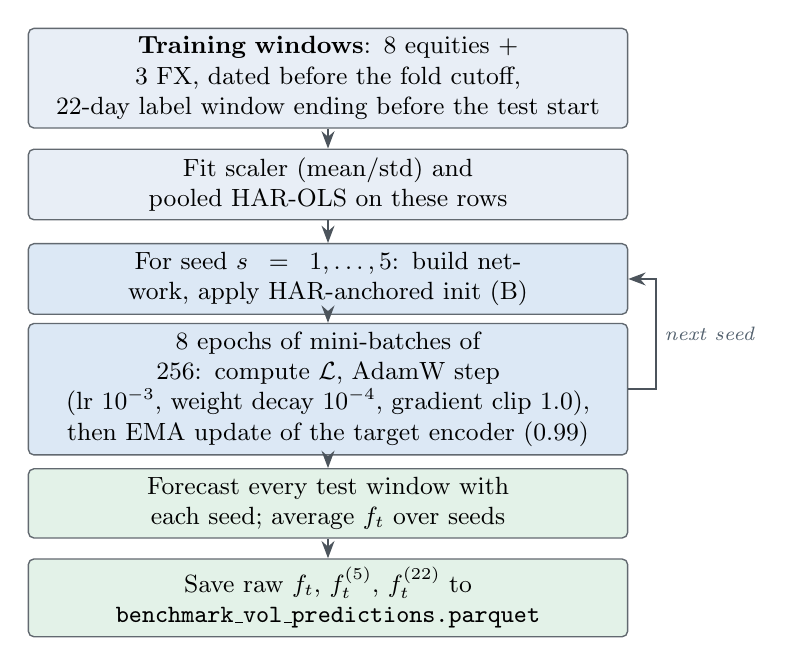
\begin{tikzpicture}[x=1cm,y=1cm]
\tikzset{st/.style={box, text width=7.4cm, minimum height=8mm}}
\node[st, fill=inp] (s1) at (0,0) {\textbf{Training windows}: 8 equities + 3 FX, dated before the fold cutoff,\\22-day label window ending before the test start};
\node[st, fill=inp] (s2) at (0,-1.35) {Fit scaler (mean/std) and pooled HAR-OLS on these rows};
\node[st, fill=enc] (s3) at (0,-2.55) {For seed $s=1,\dots,\Seeds$: build network, apply HAR-anchored init (B)};
\node[st, fill=enc] (s4) at (0,-3.95) {\Epochs\ epochs of mini-batches of 256: compute $\mathcal{L}$, AdamW step\\(lr $10^{-3}$, weight decay $10^{-4}$, gradient clip 1.0),\\then EMA update of the target encoder (0.99)};
\node[st, fill=head] (s5) at (0,-5.4) {Forecast every test window with each seed; average $f_t$ over seeds};
\node[st, fill=head] (s6) at (0,-6.6) {Save raw $f_t$, $f^{(5)}_t$, $f^{(22)}_t$ to \texttt{benchmark\_vol\_predictions.parquet}};
\draw[arr] (s1)--(s2); \draw[arr] (s2)--(s3); \draw[arr] (s3)--(s4); \draw[arr] (s4)--(s5); \draw[arr] (s5)--(s6);
\draw[arr] (s4.east) -- ++(0.35,0) |- (s3.east);
\node[dim, anchor=west] at (4.15,-3.25) {next seed};
\end{tikzpicture}

\vspace{5mm}
{\bfseries\color{accent} D. M0 configuration (exact values from the code)}\\[1mm]
{\small
\begin{tabular}{@{}p{5.1cm}l@{}}
Input window / features & 32 days / 15 \\
Model width / SSM state / SSM blocks & 64 / 64 / 2 \\
Dropout & 0.1 \\
Loss weights: QLIKE, auxiliary, SIGReg, JEPA & 1, 0.3, 0.5, 1.0 \\
EMA rate of the target encoder & 0.99 \\
Optimizer & AdamW, lr $10^{-3}$, wd $10^{-4}$ \\
Batch / epochs / gradient clip & 256 / \Epochs\ / 1.0 \\
Seeds per fold & \Seeds \\
\end{tabular}}
\end{minipage}

\newpage
% =====================================================================================
% PAGE 3 -- end-to-end system
% =====================================================================================
\noindent{\Large\bfseries\color{accent} End-to-end system: data, walk-forward benchmark, scoring, tail risk, forward test}\\[1pt]
{\small\color{muted} Each block names the script that implements it. Forecasts are saved before any metric is computed,
so every reported number is recomputed from saved files.}

\vspace{2mm}
\begin{center}
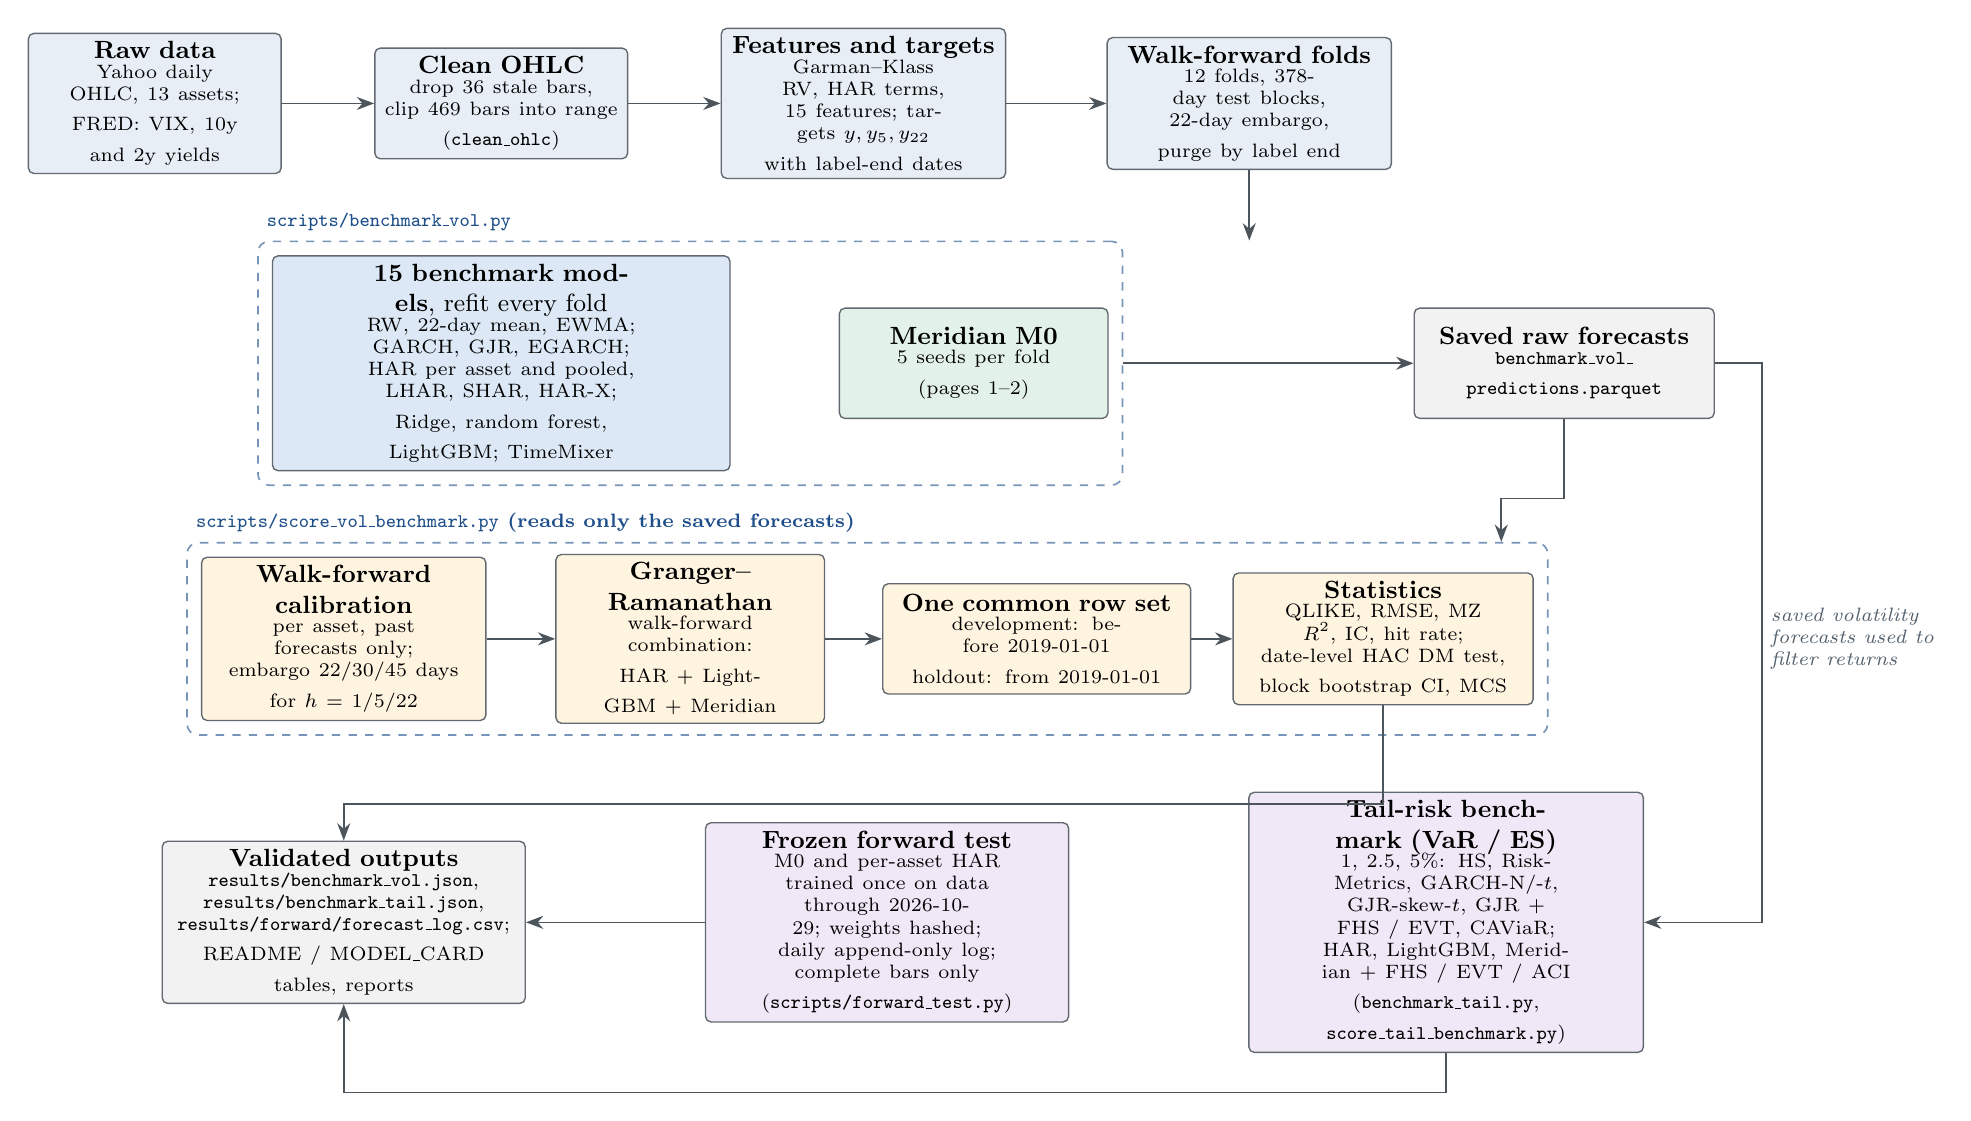
\begin{tikzpicture}[x=1cm,y=1cm]
\tikzset{b/.style={box, minimum height=14mm}}
% row 1
\node[b, fill=inp, text width=3.0cm] (src) at (0,0) {\textbf{Raw data}\sub{Yahoo daily OHLC, 13 assets;\\FRED: VIX, 10y and 2y yields}};
\node[b, fill=inp, text width=3.0cm] (clean) at (4.4,0) {\textbf{Clean OHLC}\sub{drop \NStale\ stale bars,\\clip \NClipped\ bars into range\\(\texttt{clean\_ohlc})}};
\node[b, fill=inp, text width=3.4cm] (feat) at (9.0,0) {\textbf{Features and targets}\sub{Garman--Klass RV, HAR terms,\\15 features; targets $y,y_5,y_{22}$\\with label-end dates}};
\node[b, fill=inp, text width=3.4cm] (wf) at (13.9,0) {\textbf{Walk-forward folds}\sub{\Folds\ folds, \TestDays-day test blocks,\\\EmbargoDays-day embargo,\\purge by label end}};
\draw[arr] (src)--(clean); \draw[arr] (clean)--(feat); \draw[arr] (feat)--(wf);

% row 2
\node[b, fill=enc, text width=5.6cm] (bm) at (4.4,-3.3) {\textbf{15 benchmark models}, refit every fold\sub{RW, 22-day mean, EWMA; GARCH, GJR, EGARCH;\\HAR per asset and pooled, LHAR, SHAR, HAR-X;\\Ridge, random forest, LightGBM; TimeMixer}};
\node[b, fill=head, text width=3.2cm] (mer) at (10.4,-3.3) {\textbf{Meridian M0}\sub{\Seeds\ seeds per fold\\(pages 1--2)}};
\node[b, fill=grey, text width=3.6cm] (pred) at (17.9,-3.3) {\textbf{Saved raw forecasts}\sub{\texttt{benchmark\_vol\_}\\\texttt{predictions.parquet}}};
\begin{scope}[on background layer]
\node[group, fit=(bm)(mer), inner sep=5pt] (gen) {};
\end{scope}
\node[ttl, anchor=south west] at (gen.north west) {\texttt{scripts/benchmark\_vol.py}};
\draw[arr] (wf.south) -- (wf.south |- gen.north);
\draw[arr] (gen.east) -- (pred.west);

% row 3: scoring
\node[b, fill=aux, text width=3.4cm] (cal) at (2.4,-6.8) {\textbf{Walk-forward calibration}\sub{per asset, past forecasts only;\\embargo 22/30/45 days\\for $h$ = 1/5/22}};
\node[b, fill=aux, text width=3.2cm] (gr) at (6.8,-6.8) {\textbf{Granger--Ramanathan}\sub{walk-forward combination:\\HAR + LightGBM + Meridian}};
\node[b, fill=aux, text width=3.7cm] (split) at (11.2,-6.8) {\textbf{One common row set}\sub{development: before 2019-01-01\\holdout: from 2019-01-01}};
\node[b, fill=aux, text width=3.6cm] (st) at (15.6,-6.8) {\textbf{Statistics}\sub{QLIKE, RMSE, MZ $R^2$, IC, hit rate;\\date-level HAC DM test,\\block bootstrap CI, MCS}};
\begin{scope}[on background layer]
\node[group, fit=(cal)(st), inner sep=5pt] (scg) {};
\end{scope}
\node[ttl, anchor=south west] at (scg.north west) {\texttt{scripts/score\_vol\_benchmark.py} (reads only the saved forecasts)};
\draw[arr] (cal)--(gr); \draw[arr] (gr)--(split); \draw[arr] (split)--(st);
\draw[arr] (pred.south) |- ($(scg.north east)+(-0.6,0.55)$) -- ($(scg.north east)+(-0.6,0)$);

% row 4
\node[b, fill=grey, text width=4.4cm] (out) at (2.4,-10.4) {\textbf{Validated outputs}\sub{\texttt{results/benchmark\_vol.json},\\\texttt{results/benchmark\_tail.json},\\\texttt{results/forward/forecast\_log.csv};\\README / MODEL\_CARD tables, reports}};
\node[b, fill=jepa, text width=4.4cm] (fwd) at (9.3,-10.4) {\textbf{Frozen forward test}\sub{M0 and per-asset HAR trained once on data\\through \FwdTrainThrough; weights hashed;\\daily append-only log; complete bars only\\(\texttt{scripts/forward\_test.py})}};
\node[b, fill=jepa, text width=4.8cm] (tail) at (16.4,-10.4) {\textbf{Tail-risk benchmark (VaR / ES)}\sub{1, 2.5, 5\%: HS, RiskMetrics, GARCH-N/-$t$,\\GJR-skew-$t$, GJR + FHS / EVT, CAViaR;\\HAR, LightGBM, Meridian + FHS / EVT / ACI\\(\texttt{benchmark\_tail.py}, \texttt{score\_tail\_benchmark.py})}};
\draw[arr] (pred.east) -- ++(0.6,0) |- (tail.east);
\node[dim, anchor=west, align=left] at (20.4,-6.8) {saved volatility\\forecasts used to\\filter returns};
\draw[arr] (st.south) -- (st.south |- 0,-8.9) -| (out.north);
\draw[arr] (fwd.west) -- (out.east);
\draw[arr] (tail.south) -- ++(0,-0.5) -| (out.south);
\end{tikzpicture}
\end{center}

\vspace{1mm}
{\small\noindent\textbf{Leakage controls, enforced in code and checked by \NTests\ automated tests.} Every scaler, regression
and network is fit on rows dated before the fold cutoff whose label window ends before the test start; calibration and
combination use only past forecasts; a tail forecast for day $t{+}1$ uses standardized returns of earlier days only;
all model choices use the development period only; the forward test logs a forecast before its target day exists.}

\end{document}
